\documentclass{article}
\usepackage{graphicx}
\usepackage{float}
\begin{document}
\title{Malwares for Use cases for EMI measurements}
\author{Abhinav Narain}
\maketitle

\section{Purpose}
The purpose of the document is to define two states of affairs finding
real malware/botnets which can be used for the project. We have to
show real world workloads to be captured.

\section{Nest Camera}
\begin{enumerate}
\item The camera signals are not very prominent
\item 
\end{enumerate}

\begin{figure}[t!]
\centering
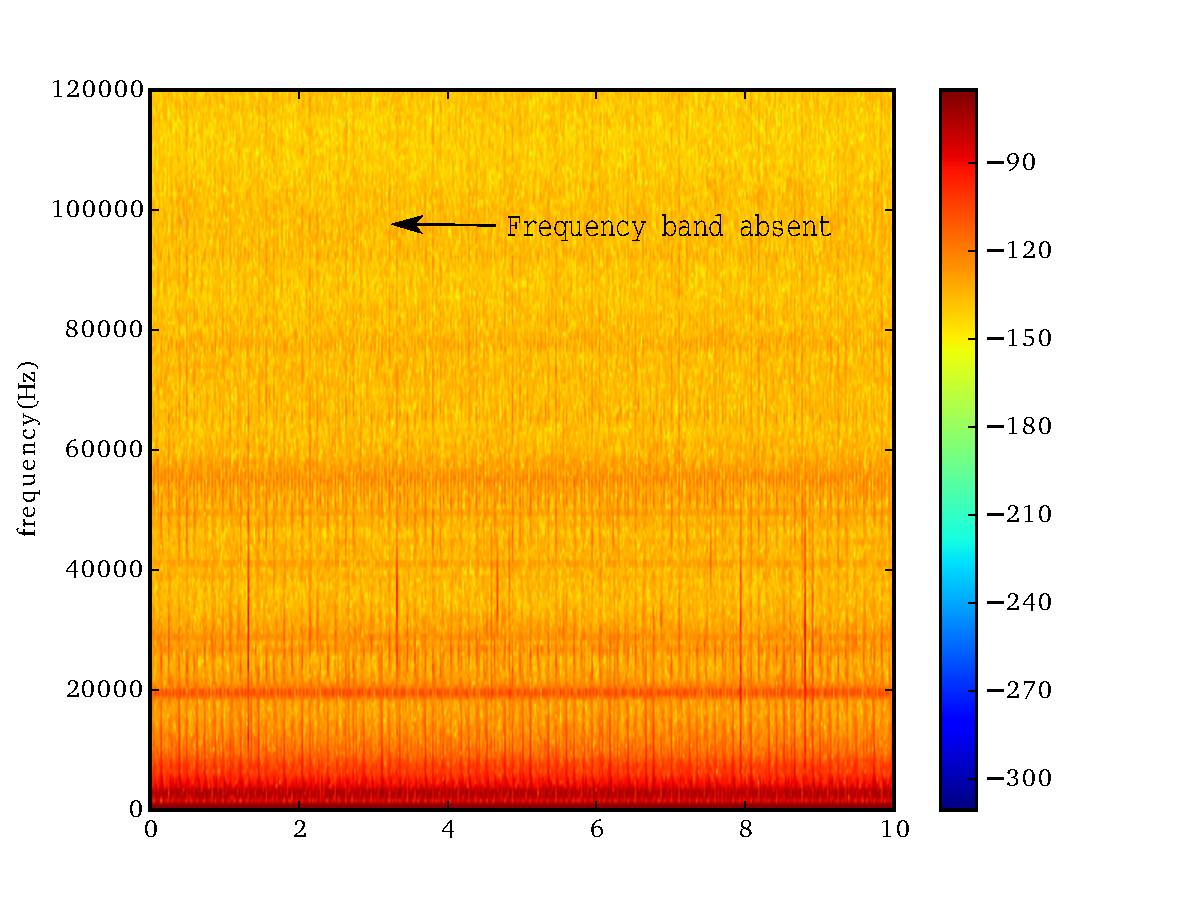
\includegraphics[width=\linewidth]{./figures/nest_standby_4096_clipped.pdf}
\caption{}
\label{fig:rasp}
\end{figure}

\begin{figure}[t!]
\centering
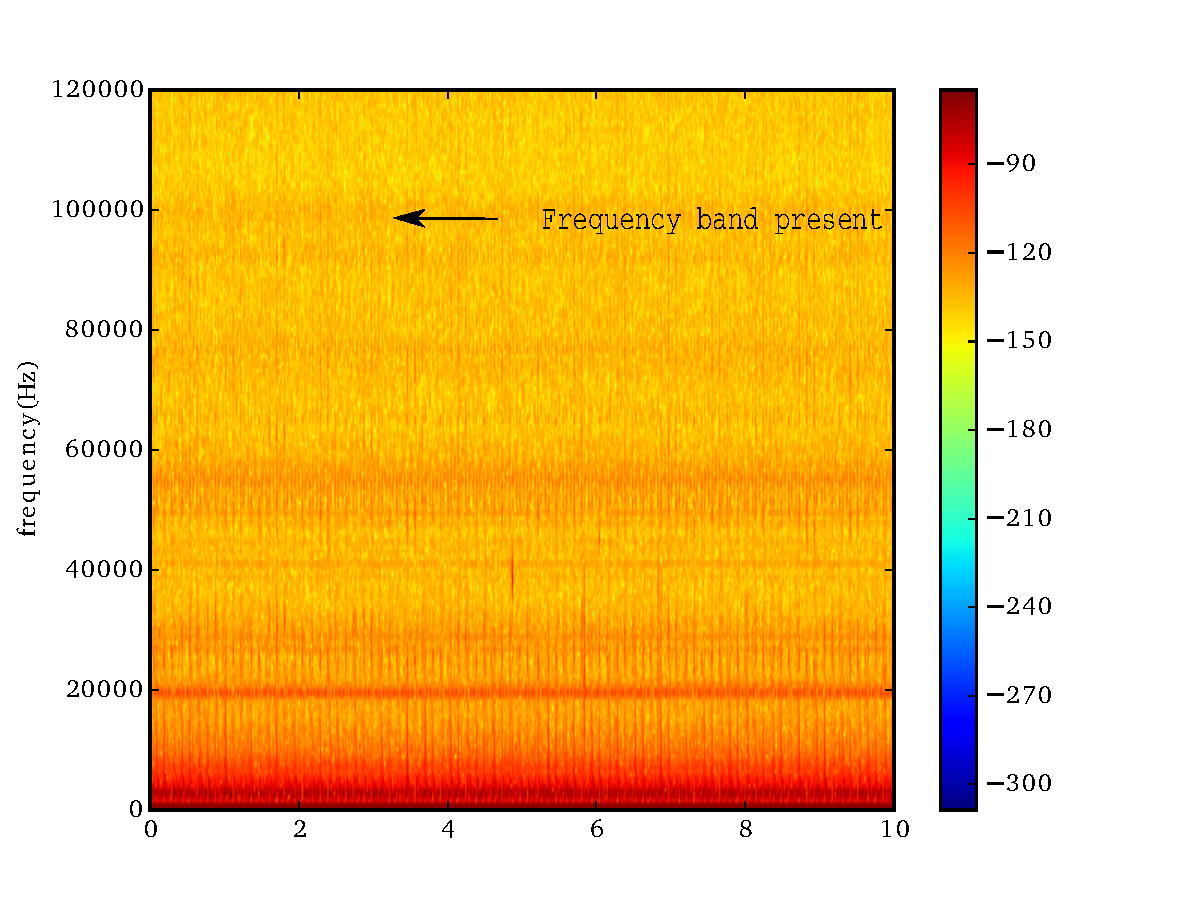
\includegraphics[width=\linewidth]{./figures/nest_stream1080_4096_clipped.pdf}
\caption{}
\label{fig:rasp}
\end{figure}

\begin{figure}[t!]
\centering
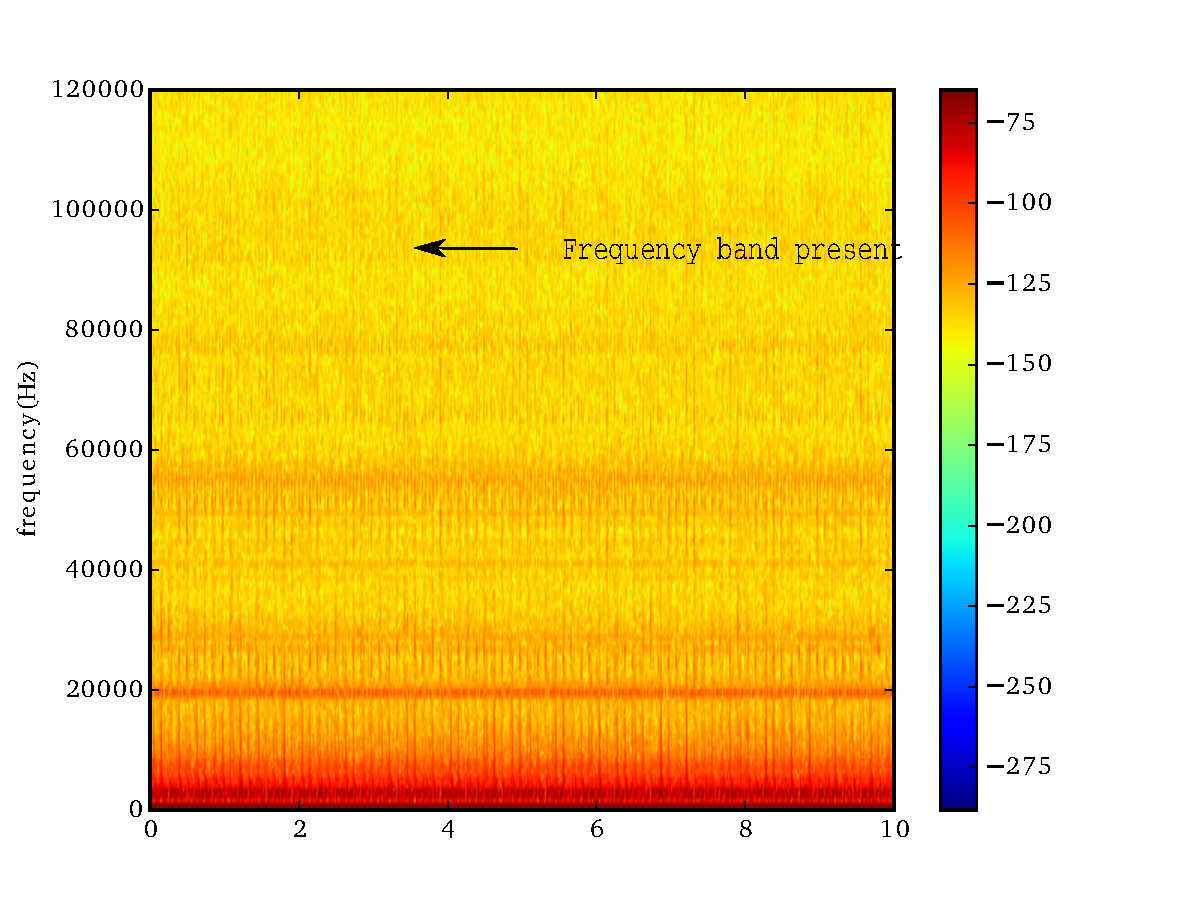
\includegraphics[width=\linewidth]{./figures/nest_stream_4096_clipped.pdf}
\caption{}
\label{fig:rasp}
\end{figure}


\section{Alexa}
\begin{enumerate}
\item The frequency 
\item 
\end{enumerate}
Alexa is a fairly complex device to be modelled. 
I have not been very successful with showing Alexa and Nest Camera in
different states, suggesting the hardware 
Alexa is always listening and Only when you mention "Alexa, do the
following" it connects to the Internet I have tried few experiments
with Alexa when it

\begin{figure}[t!]
\centering
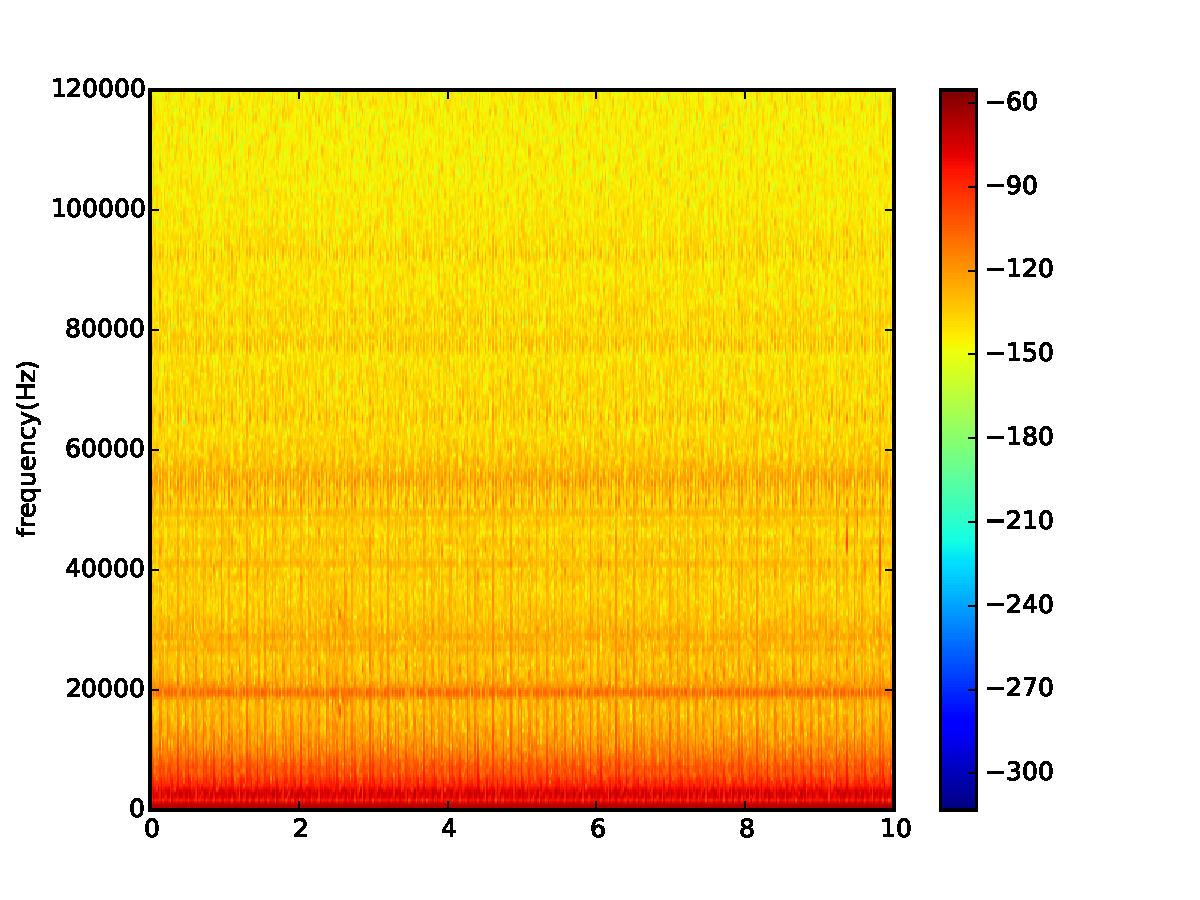
\includegraphics[width=\linewidth]{./figures/alexaMusic_4096_clipped.pdf}
\caption{EMI generated by Amazon Echo Alexa when it is playing music from the Internet. Fs=2.5MHz, N=4096, Fs/N=610.35}
\label{fig:alexaMusic}
\end{figure}

\begin{figure}[t!]
\centering
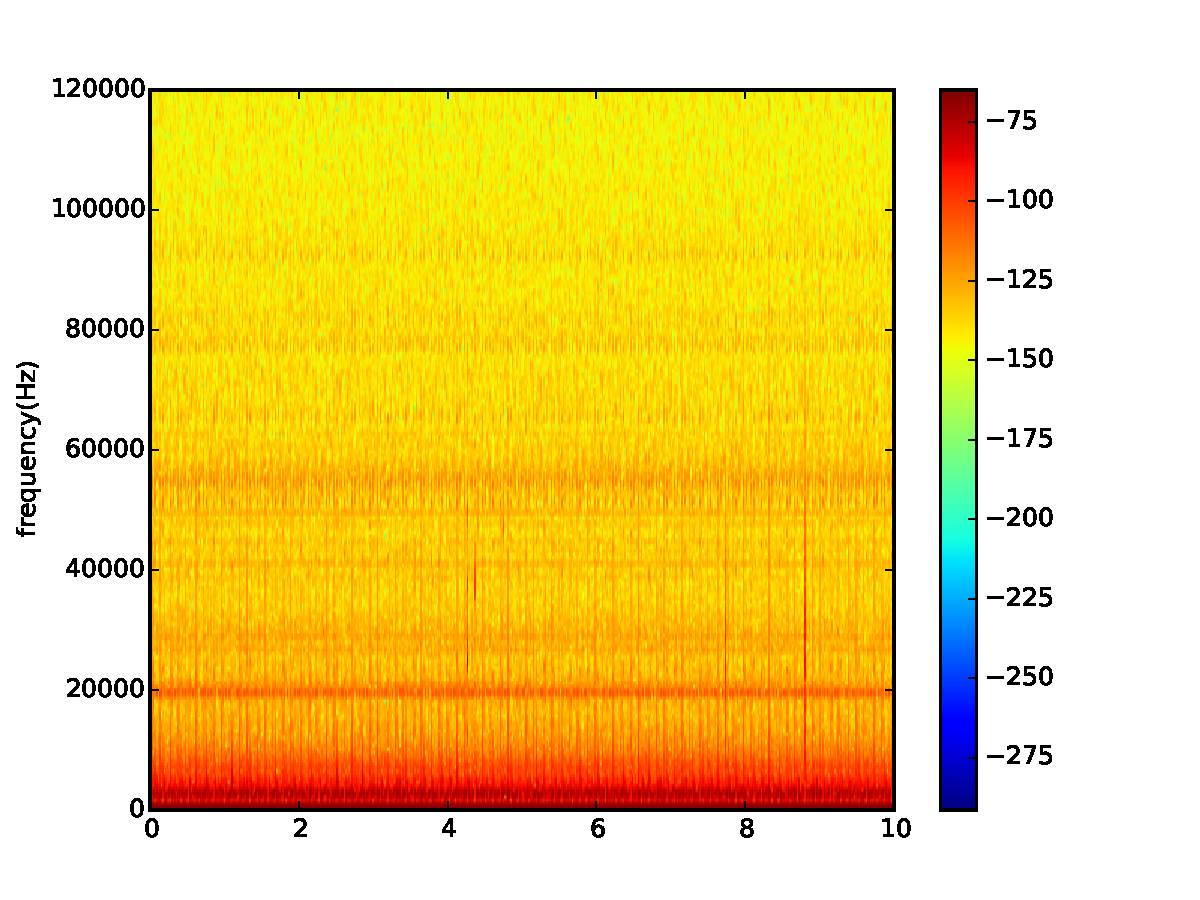
\includegraphics[width=\linewidth]{./figures/alexaOff_4096_clipped.pdf}
\caption{EMI generated by Amazon Echo Alexa when it is not asked for any task and is idle. Fs=2.5MHz, N=4096, Fs/N=610.35}
\label{fig:alexaoff}
\end{figure}

\begin{figure}[t!]
\centering
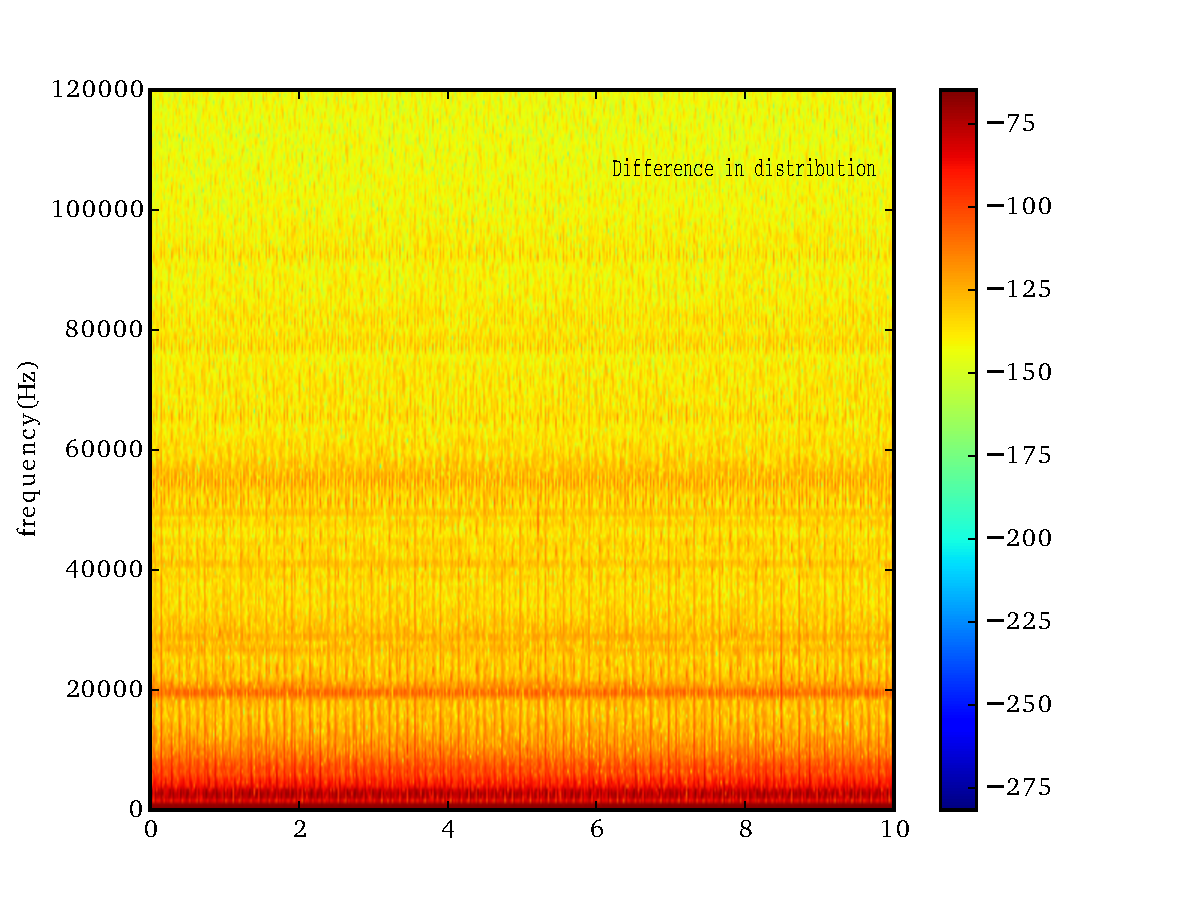
\includegraphics[width=\linewidth]{./figures/alexaSearch_4096_clipped.pdf}
\caption{EMI generated by Amazon Echo Alexa when it is listening to a query to search on the Internet. Fs=2.5MHz, N=4096, Fs/N=610.35}
\label{fig:alexaSearch}
\end{figure}

\section{IoT Botnet samples for Evaluation}

\begin{enumerate}
\item Linux.Darlloz (mines Crypto Currency such as DogeCoin, MinCoins)
\item Linux.Remaiten (CNC by actual IRC channel)
\item Linux/IRC Telnet (IRC is the CNC)
\item *Linux.Wifatch (expected to secure IoT, turned rogue)
\item Linux/Luabot (Botnet written in \textit{Lua})
\item *Linux Aidra
\end{enumerate}

I have been able to get source code for two of the above malwares,
although they do not compile.

\subsection{Mining botnets}
I have searched for different IoT botnets. There has been a specific attack vector of mining crypto
currencies on \textit{Hikvision DVR}s in 2013-2014. Currencies such as
\textit{Dogecoin, MinCoin and LiteCoin} have been mined~[4] by some bots only
on x86 (It has not been observed on ARM or MIPS architectures). Most
of the attacks have been DDoS otherwise.

\begin{figure}[t!]
\centering
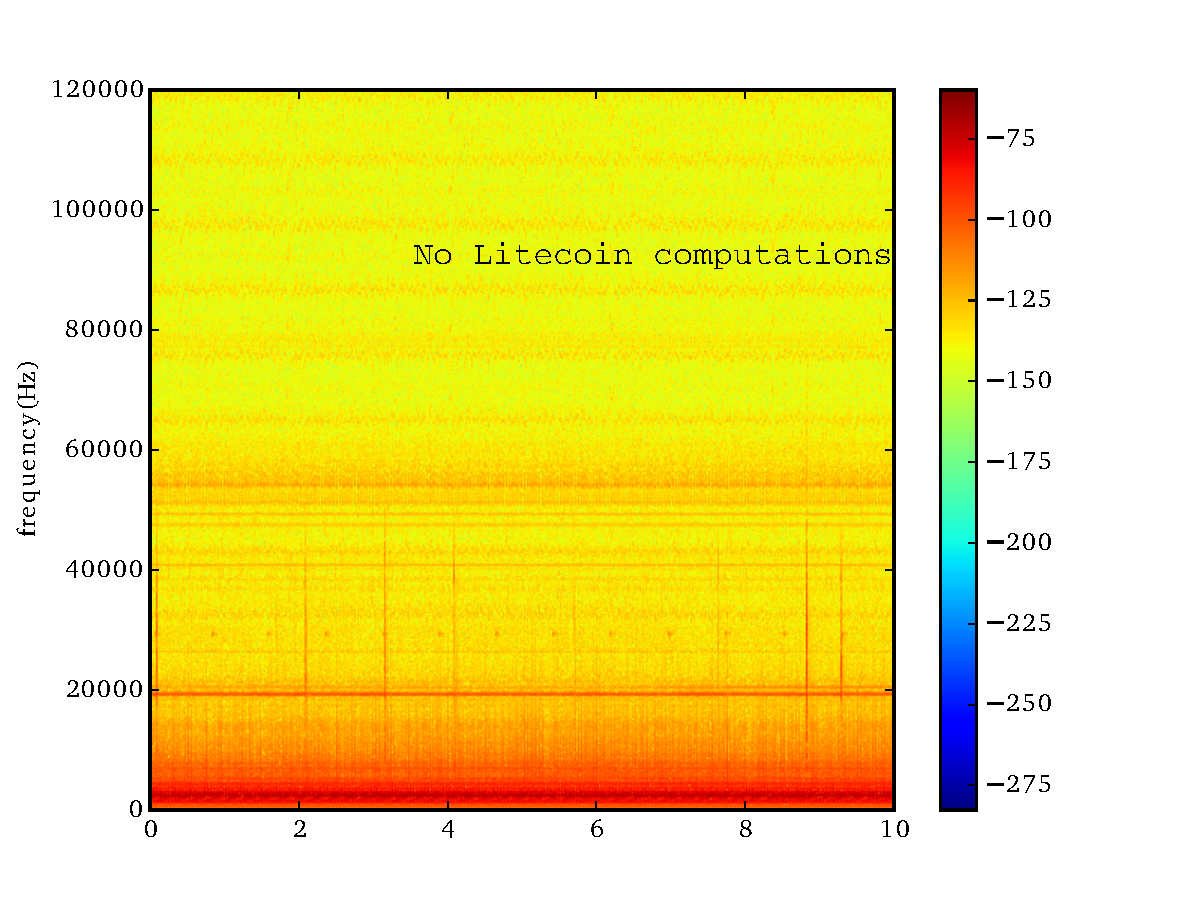
\includegraphics[width=\linewidth]{./figures/litecoin_stopped_4096_clipped.pdf}
\caption{Raspberry Pi Idle for baseline comparison}
\label{fig:raspi_litecoinOff}
\end{figure}

\begin{figure}[t!]
\centering
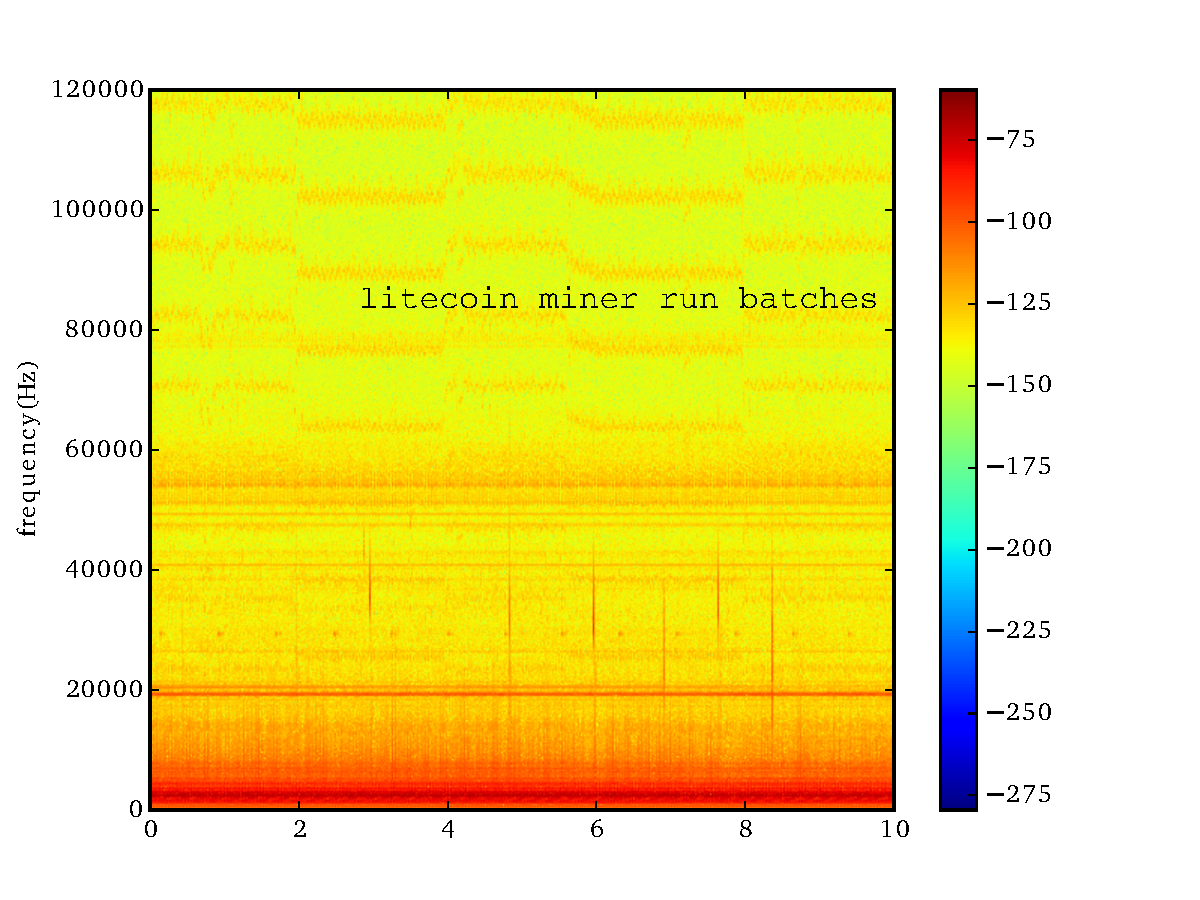
\includegraphics[width=\linewidth]{./figures/litecoin_working_4096_clipped.pdf}
\caption{Raspberry Pi running proof-of-work computations for crypto-currency using a litecoin client connected to a remote server}
\label{fig:raspi_litecoinOn}
\end{figure}


\subsection{Comments}
\begin{enumerate}
\item It has been difficult to find a working codebase like Mirai
  which can be run on OpenWrt router or Raspberry Pi for analysis
\item There are parts of the IoT malware binaries~[2,3] which are
  reversed engineered to show the exploit but are not good to run on
  raspberry or router
\item Number of malware github repositories have worms targetting
  Windows. WattsUpDoc(Kevin Fu et. al) had Windows device (compounder)
  which I suppose were able to use such malwares
\item Able to run \textbf{cpuminer}, a mining software on CPUs for
  bitcoins instead other digital currencies. Unclear(shouted out
  to OpenWrt folks without response) how to port it on OpenWrt.
\item I contacted a reverse-engineer/hacker who pointed
  \textit{KernelMode.info} forum for binaries for
  \textit{Linux/LuaBot} malware. Unfortunately, I am not getting
  registered to login the forum. Unclear to proceed.  
\end{enumerate}

\section{References}
\begin{enumerate}
\item https://spqr.eecs.umich.edu/papers/clark-healthtech13.pdf
\item https://w00tsec.blogspot.com/2016/09/luabot-malware-targeting-cable-modems.html
\item http://blog.malwaremustdie.org/2016/09/mmd-0057-2016-new-elf-botnet-linuxluabot.html
\item https://securityledger.com/2014/03/linux-iot-worm-still-alive-and-mining-virtual-coins/
\end{enumerate}

\section{Supplementary}

\section{Power, Current, Voltage consumed by Nest Camera}
\begin{figure}[H]
\centering
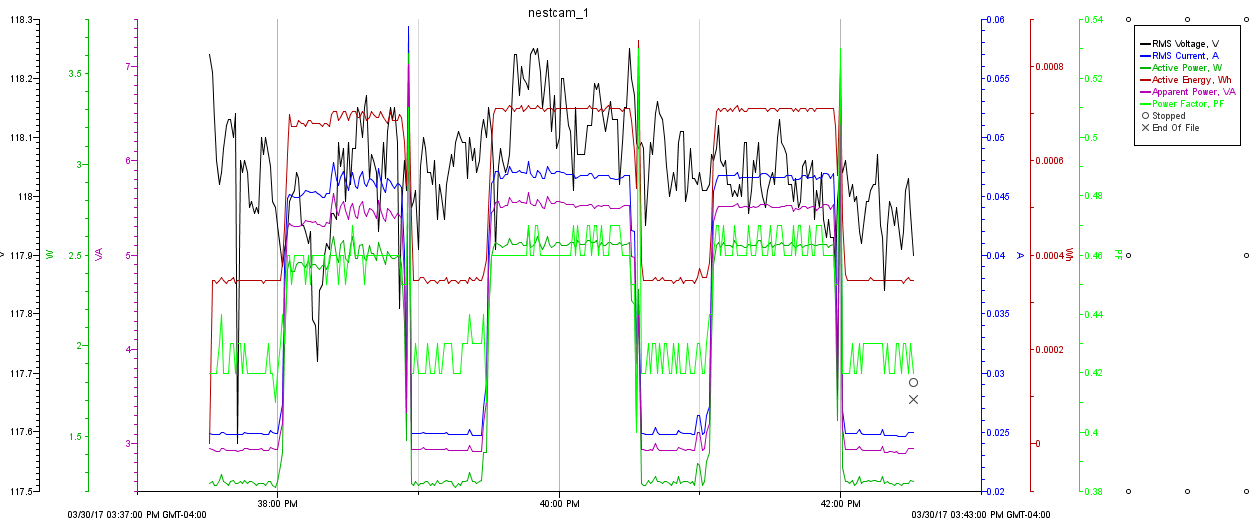
\includegraphics[width=\textwidth]{./figures/nestcam_experiment.PNG}
\caption{Actual Power consumed by Nest Camera when Turned On and
  Turned Off. Generated by experiments done by student working on
  Power Consumption project}
\label{fig:powerConNest}
\end{figure}
I have borrowed this image(generated by software provided by Power
measurement equipment) from an undergraduate student working on actual
power measurements with IoT devices while he conducted experiments
with Nest Camera. It shows good variation in Current and Energy
consumptions (voltage is not clearly indicative) when the Camera is
turned for streaming and when it is not streaming.

\subsection{Network access denied}
My wall Ethernet-port is blocked at times by Princeton support as they
detect malware!
\begin{verbatim}
Name: pu153716
DNS Domain: student.Princeton.EDU
Entry Type: HOST
Interface[1] Type: Ethernet
Interface[1] MACaddress: e8:de:27:b7:24:4b
Interface[1] Subnet: driftnet
Interface[1] IPAddress: 172.24.63.68
System Type: OTHER
Operating System: LINUX
OIT NIS NetGroup: princetonhosts
OIT NIS NetGroup: princetonunixhosts
Technical Contact: heekang@princeton.edu
Dormnet Subscriber Netid: heekang

``Mirai is malware that turns computer systems running Linux into
remotely controlled ``bots'', that can be used as part of a botnet in
large-scale network attacks.'' en.wikipedia.org/wiki/Mirai_(malware)
\end{verbatim}

\end{document}
